\documentclass{beamer}
\usepackage{./common_slides}
\usepackage[absolute,overlay]{textpos}
\usepackage{graphicx}


\title{ Distributed Stochastic Gradient Descent }

\author{Kevin Yang and Michael Farrell}
\begin{document}

\begin{frame}
  \titlepage
\end{frame}

\begin{frame}{Motivation - Deep Learning}

\begin{columns}[T] % align columns
\begin{column}{.48\textwidth}
\begin{itemize}
\item Deep-Learning
\begin{itemize}
\item Objective: Learn a complicated, non-linear function that minimzes some loss function
\end{itemize}
\item Why do we need deep models?
\begin{itemize}
\item The class of linear functions is inadequate for many problems.
\end{itemize}
\end{itemize}
\end{column}%
\hfill%
\begin{column}{.48\textwidth}
\begin{figure}
    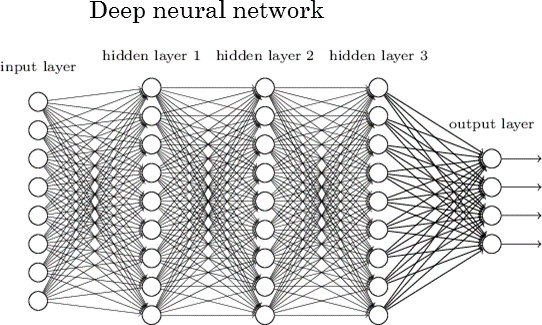
\includegraphics[scale = .35]{./img/deep_learning}
      \caption{\scalebox{.3}{http://www.rsipvision.com/exploring-deep-learning/}}
\end{figure}
\begin{figure}
    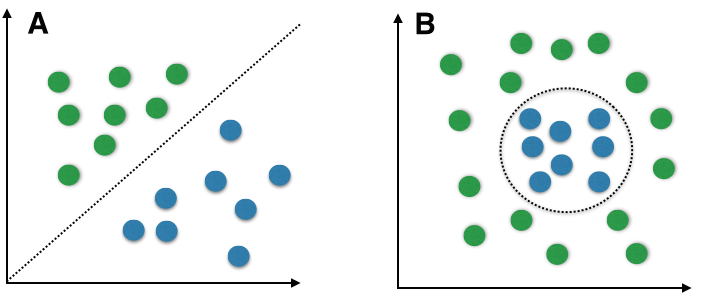
\includegraphics[scale = .17]{./img/lin_v_nonlin}
      \caption{\scalebox{.3}{http://sebastianraschka.com/Articles/2014{\_}naive{\_}bayes{\_}1.html}}
\end{figure}
\end{column}%
\end{columns}
\end{frame}

\begin{frame}{Motivation - Deep Learning}
\begin{itemize}
\item How do we learn these deep models?
\begin{itemize}
\item Choose a random example
\item Run the neural network on the example
\item Adjust the parameters of the network such that our loss function is minimized more than it was before
\item Repeat
\end{itemize}
\pause
\item Difficulties?
\begin{itemize}
\item Local Minima
\item Non-convexity
\item Neural Networks can have millions or even billions of parameters
\end{itemize}
\end{itemize}
\begin{textblock*}{5cm}(8cm,.5cm) % {block width} (coords)
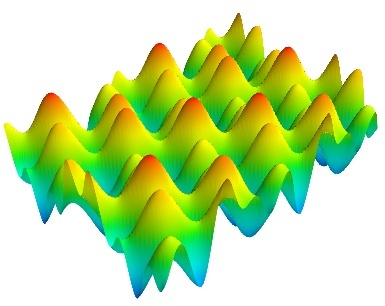
\includegraphics[scale = .3]{./img/2d_func}
\end{textblock*}
\end{frame}

\begin{frame}{Motivation - SGD}
\begin{itemize}
\item How do we maximize our reward function?
\begin{itemize}
\item One common technique is Stochastic Gradient Descent
\item $\mathbf w$ is the vector of parameters for the model
\item $\eta$ is the learning rate 
\item $\mathbf f(\mathbf w)$ is the loss function evaluated with the current parameters $\mathbf w$
\item 
\begin{algorithmic}
\State $\mathbf w \gets \mathbf 0$
\While {$\mathbf f(\mathbf w)$ is not minimized}
	\For {$i = 1, n$}
    \State $\mathbf w \gets \mathbf w - \eta\nabla f(\mathbf w)$
	\EndFor
\EndWhile

\end{algorithmic}
\item As the number of training examples, $n$, and the number of parameters, $|\mathbf w|$, increases, this algorithm quickly becomes very slow...
\end{itemize}
\end{itemize}
\end{frame}

\begin{frame}{Motivation - Distributed SGD}
\begin{itemize}
\item Since some of these models take days/weeks/months to run, we would hope that we could use a distributed computing cluster parallelize this process.
\pause
\item Learn from Google!
\begin{itemize}
\item DistBelief- 2012
\begin{itemize}
\item Downpour SGD
\item Sandblaster L-BFGS
\end{itemize}
\item TensorFlow -2015
\begin{itemize}
\item gRPC
\end{itemize}
\end{itemize}
\end{itemize}

\end{frame}

\begin{frame}{DistBelief - Downpour SGD}
\begin{itemize}
\item ``An asynchronous stochastic gradient descent procedure supporting a large number of model replicas."
\end{itemize}
$$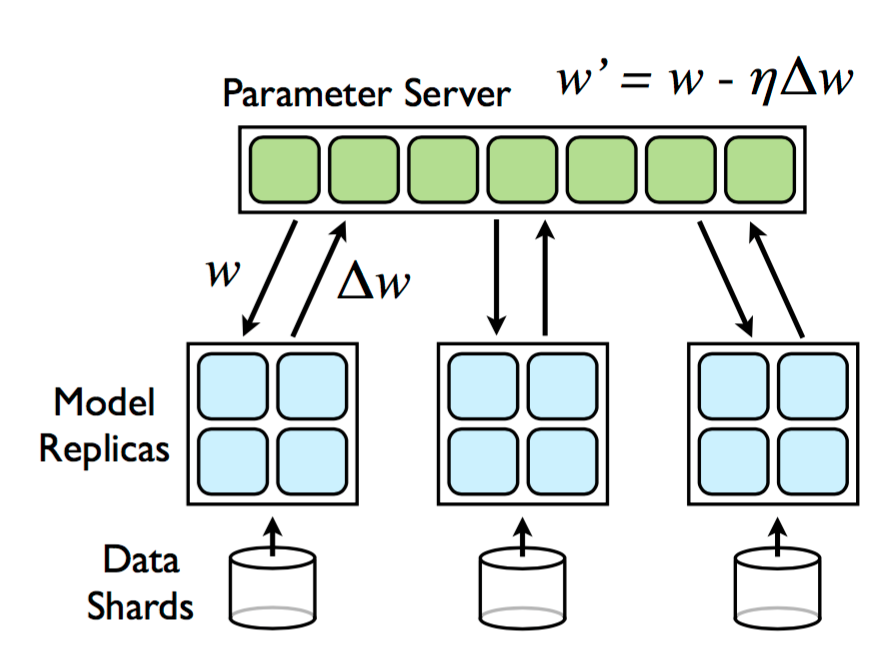
\includegraphics[scale = .5]{./img/downpour}$$
\end{frame}

\begin{frame}{DistBelief - Sandblaster L-BFGS}
\begin{itemize}
\item ``A framework that supports a variety of distributed batch optimization procedures, including a distributed implementation of L-BFGS"
\end{itemize}
$$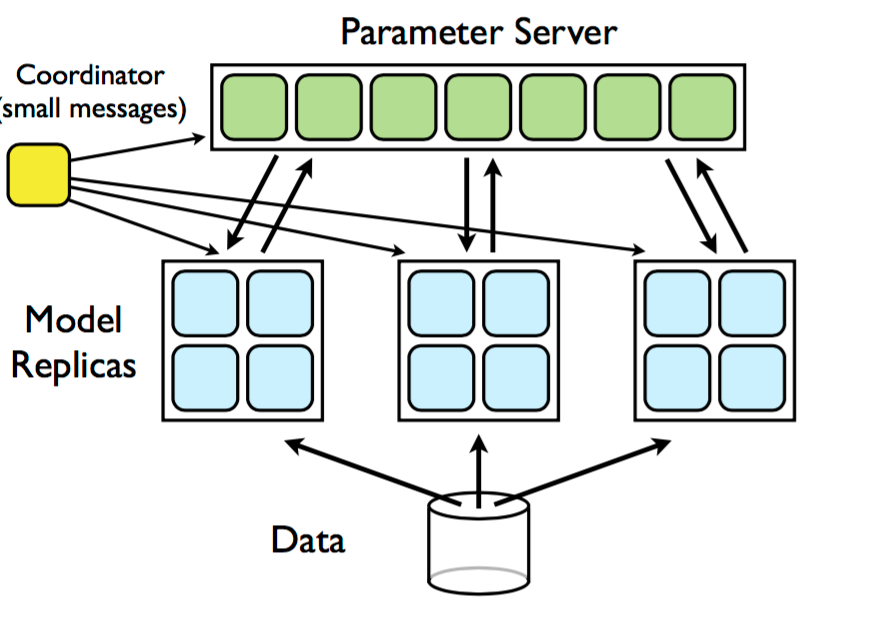
\includegraphics[scale = .5]{./img/sandblaster}$$
\end{frame}

\begin{frame}{TensorFlow-GRPC}
\begin{itemize}
\item Second Generation ML Model focused on distributing models to CPUs and GPUs
\item Uses the high performance RPC framework (GRPC) to communicated between separate processes
\begin{itemize}
\item Uses Protocol Buffers -v3
\item C-based
\item Client-server stubs in 10+ languages and counting
\end{itemize}
\end{itemize}
$$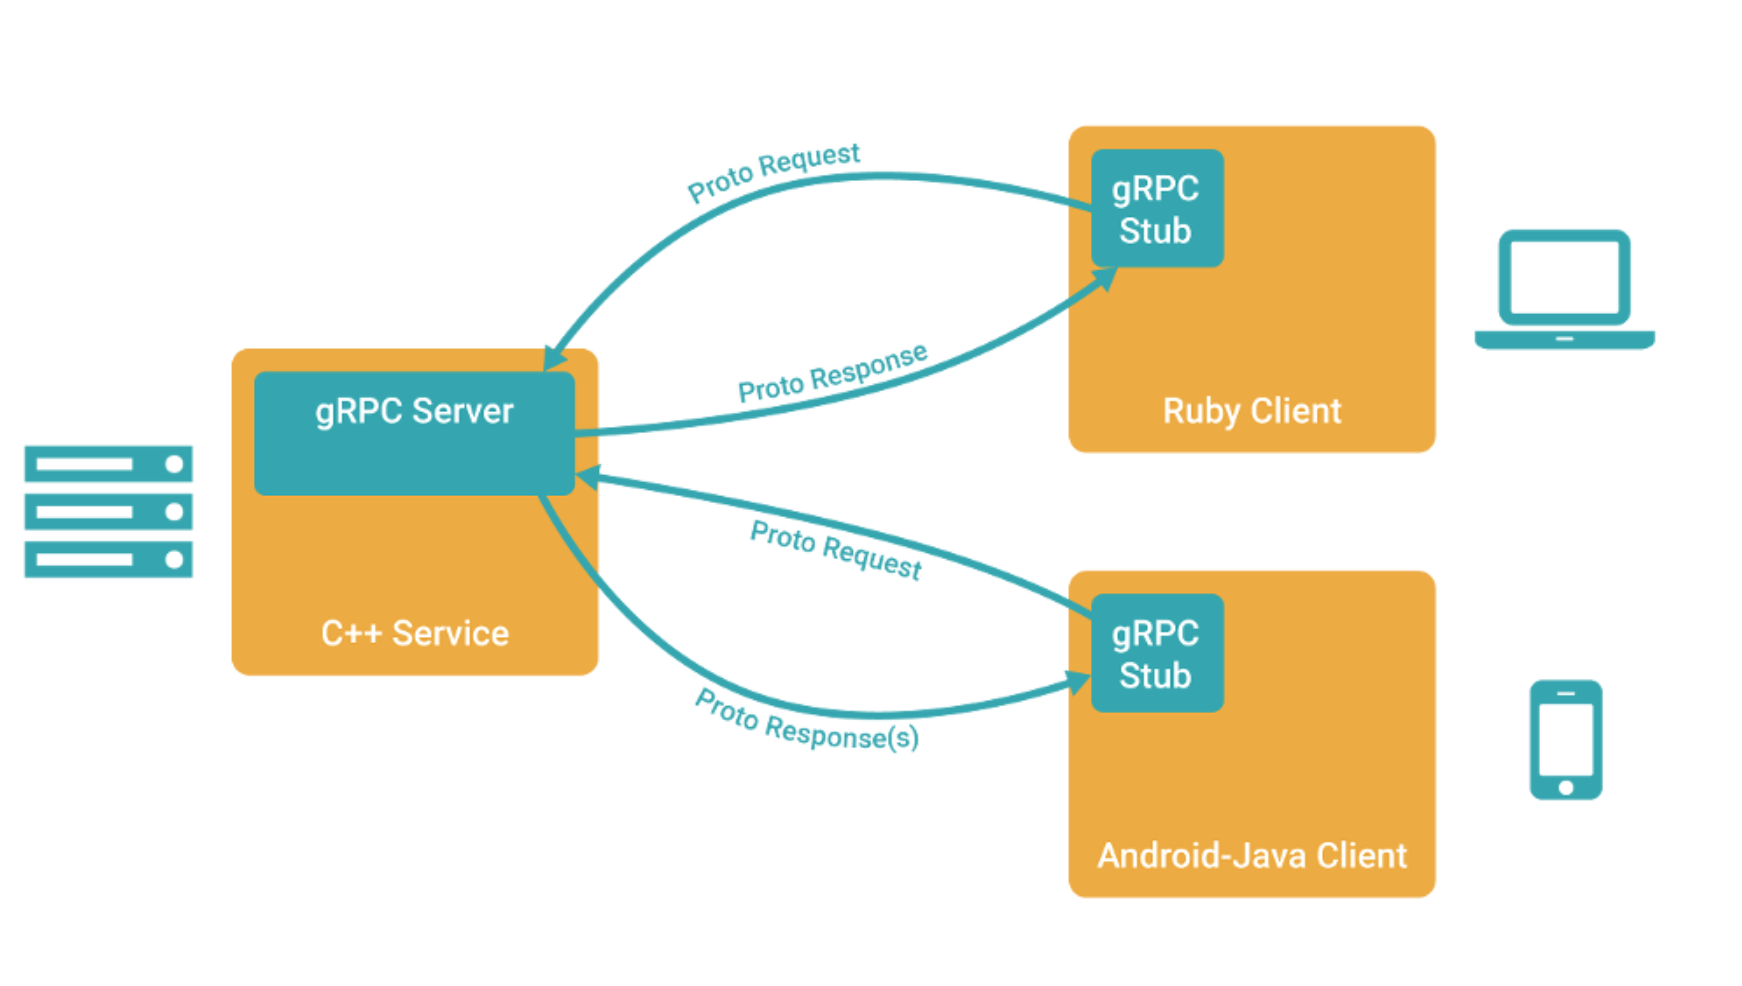
\includegraphics[scale = .2]{./img/gRPC}$$
\end{frame}

\begin{frame}{DistBelief/TensorFlow Summary}
\begin{itemize}
\item TensorFlow is basically the second version of DistBelief that is approximately twice as fast and much more user-friendly.
\item Results from DistBelief:
\end{itemize}
$$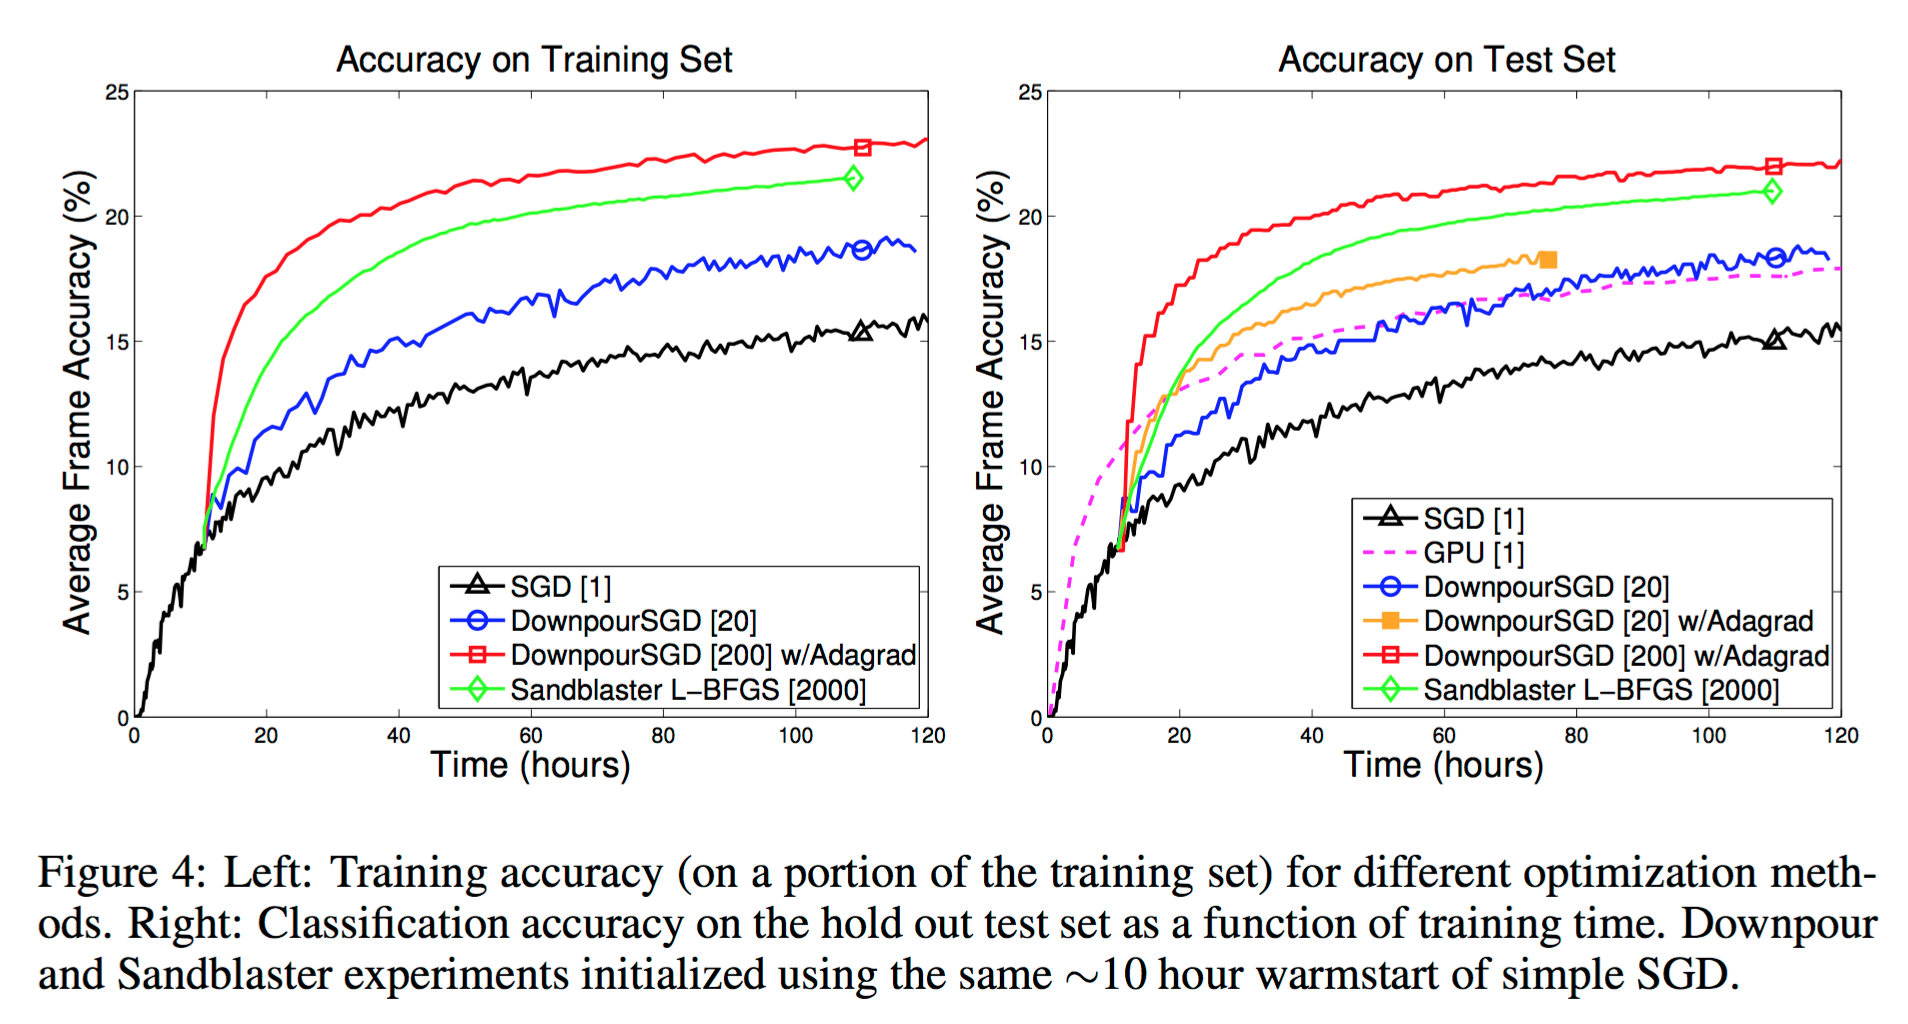
\includegraphics[scale = .18]{./img/dist_train}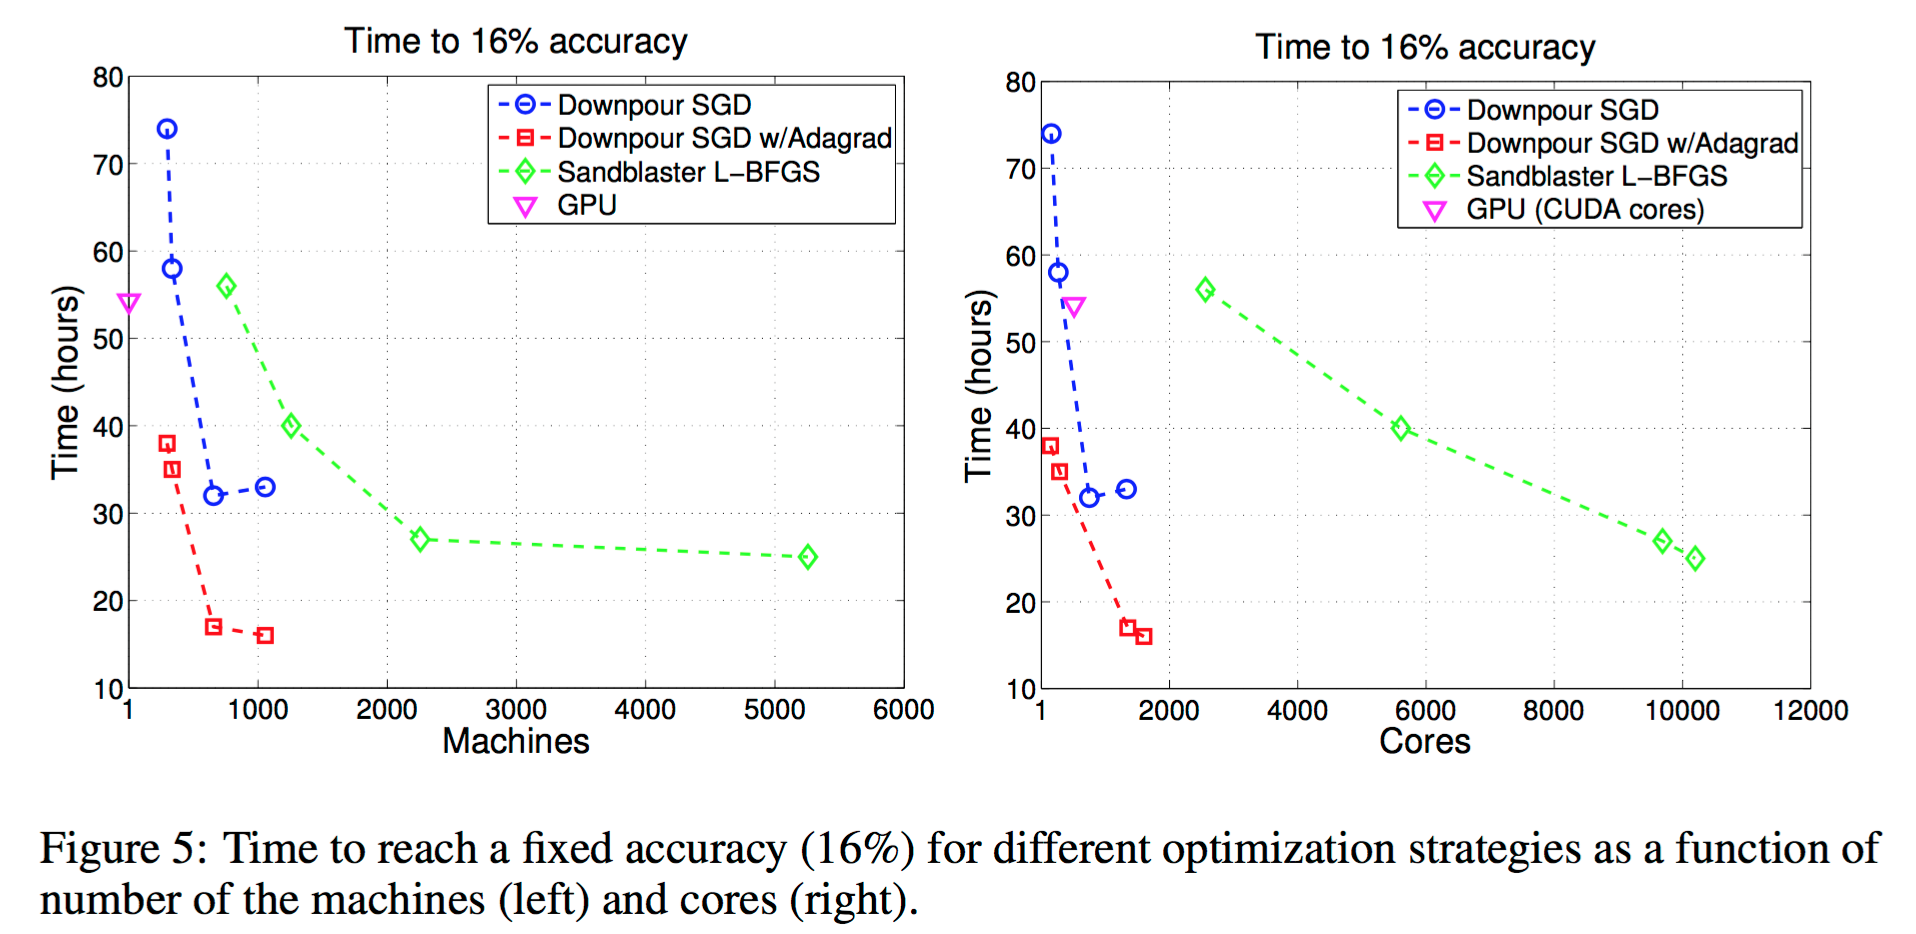
\includegraphics[scale = .18]{./img/dist_16}$$

\end{frame}

\begin{frame}{Our Project}
\begin{itemize}
\item We hope to build our own Distributed SGD model modeled based on both DistBelief and TensorFlow
\begin{itemize}
\item From TensorFlow- Use GRPC with Protocol Buffers to communicated between processes 
\item From DistBelief -Implement Downpour-SGD (the most effective model with limited resources) first, and then attempt to implement Sandblaster
\end{itemize}
\end{itemize}
\end{frame}

\begin{frame}{Our Example}
Talk about image dataset
\end{frame}

\begin{frame}{Exploration of Downpour-SGD}
\begin{itemize}
\item The Downpour-SGD requires the passing of parameters between processes
\item Bottleneck here is bandwidth 
\item Parameters in the range of 100MB-50GB
\end{itemize} 
$$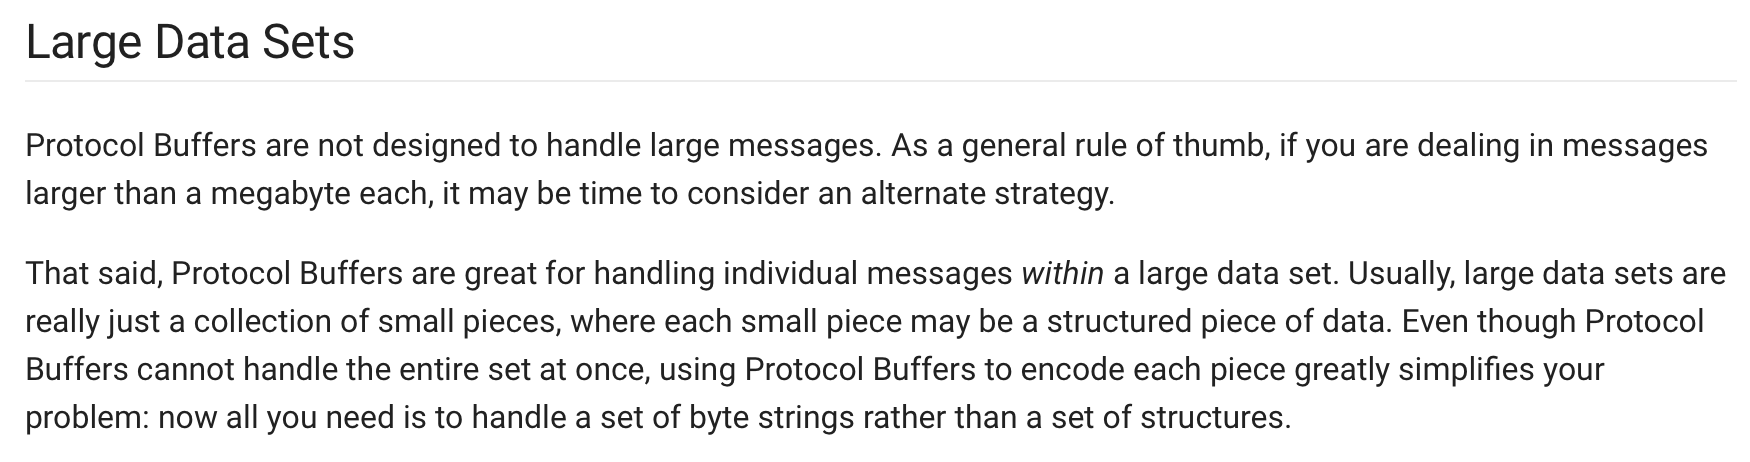
\includegraphics[scale = .27]{./img/large_data}$$

\end{frame}

\begin{frame}{Exploration of Downpour-SGD}
\begin{itemize}
\item Many of these models are extremely sparse
\begin{itemize}
\item only send parameters updated
\item only update parameters every $n_x$ times
\end{itemize}
\item Explore streaming vs single result
\item Add diagram of why streaming could be helped
\end{itemize} 
\end{frame}



\begin{frame}{Exploration of Downpour-SGD Algorithm}
\begin{itemize}
\item 
\end{itemize} 

\end{frame}


\end{document}
